\documentclass[tikz,convert={outfile=\jobname.svg}]{standalone}
\begin{document}
   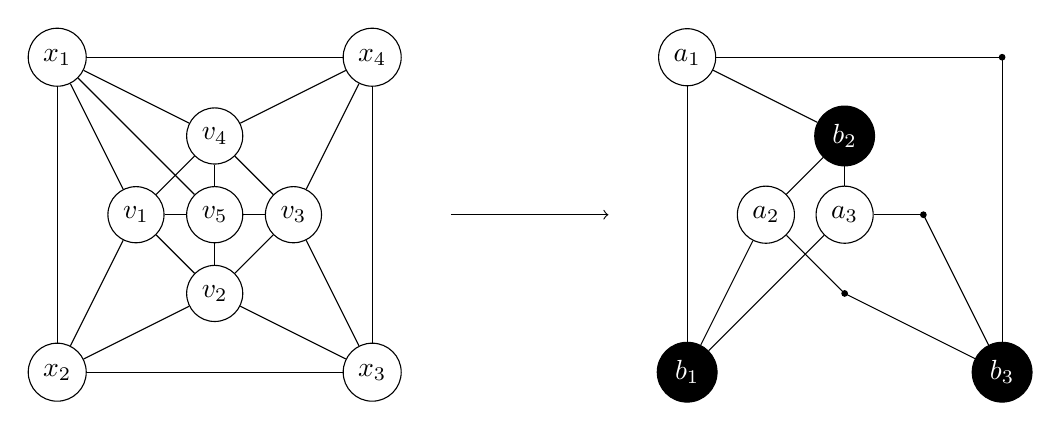
\begin{tikzpicture}
      \begin{scope}
         \def \Vertices {
            1/0/0/$x_2$,
            2/0/4/$x_1$,
            3/1/2/$v_1$,
            4/2/1/$v_2$,
            5/2/2/$v_5$,
            6/2/3/$v_4$,
            7/3/2/$v_3$,
            8/4/0/$x_3$,
            9/4/4/$x_4$}
         \def \Edges {
            1/2,
            1/3,
            1/4,
            1/8,
            2/3,
            2/5,
            2/6,
            2/9,
            3/4,
            3/5,
            3/6,
            4/5,
            4/7,
            4/8,
            5/6,
            5/7,
            6/7,
            6/9,
            7/8,
            7/9,
            8/9}
         \foreach \u / \x / \y / \n in \Vertices {
            \node[draw, circle] (\u) at (\x, \y){\n};
         }
         \foreach \u / \v in \Edges {
            \path[draw] (\u) -- (\v);
         }
      \end{scope}
      \begin{scope}[xshift=8cm]
         \def \Vu {
            u1/0/4/$a_1$,
            u2/1/2/$a_2$,
            u3/2/2/$a_3$}
         \def \Vv {
            v1/0/0/$b_1$,
            v2/2/3/$b_2$,
            v3/4/0/$b_3$}
         \foreach \no / \x / \y / \na in \Vu {
            \node[draw, circle] (\no) at (\x, \y){\na};
         }
         \foreach \no / \x / \y / \na in \Vv {
            \node[draw, circle, fill=black, text=white] (\no) at (\x, \y){\na};
         }
         \filldraw[black] (2, 1) circle (1pt);
         \filldraw[black] (3, 2) circle (1pt);
         \filldraw[black] (4, 4) circle (1pt);
         \path[draw] (u1) -- (v1);
         \path[draw] (u1) -- (v2);
         \path[draw] (u1) -- (4, 4);
         \path[draw] (4, 4) -- (v3);
         \path[draw] (u2) -- (v1);
         \path[draw] (u2) -- (v2);
         \path[draw] (u2) -- (2, 1);
         \path[draw] (2, 1) -- (v3);
         \path[draw] (u3) -- (v1);
         \path[draw] (u3) -- (v2);
         \path[draw] (u3) -- (3, 2);
         \path[draw] (3, 2) -- (v3);
      \end{scope}
      \draw[->] (5,2) -- (7,2);
   \end{tikzpicture}
\end{document}
